\documentclass[runningheads]{llncs}
%
\usepackage[T1]{fontenc}
%
\usepackage{graphicx}
%

% Daniel Motz's packages
\usepackage{etoolbox}
\makeatletter
\let\llncs@addcontentsline\addcontentsline
\patchcmd{\maketitle}{\addcontentsline}{\llncs@addcontentsline}{}{}
\patchcmd{\maketitle}{\addcontentsline}{\llncs@addcontentsline}{}{}
\patchcmd{\maketitle}{\addcontentsline}{\llncs@addcontentsline}{}{}
\setcounter{tocdepth}{3}
\makeatother
\usepackage{bookmark}

\usepackage{amsfonts}
\usepackage{amsmath}
\usepackage{stmaryrd}
\usepackage{amssymb}
\usepackage{mathtools}
\usepackage{ bbold }
\DeclarePairedDelimiter\ceil{\lceil}{\rceil}
\DeclarePairedDelimiter\floor{\lfloor}{\rfloor}

\usepackage{tikz}
\usepackage{tikz-3dplot}
\usepackage{pgfplots}
\pgfplotsset{compat = newest}

\usepackage{hyperref}

\usepackage{setspace}
\doublespacing

\renewcommand{\abstractname}{}
\newcommand{\inline}{\mintinline[fontsize=\normalsize]{c++}{text}}
\DeclareUnicodeCharacter{03BB}{$\lambda$}
% END Daniel Motz's packages

\begin{document}
%
\title{
    Automaten und Berechenbarkeit \\
    Dr. Jörg Vogel \\
    Skript zur VL im WS 2021
}
%
\titlerunning{
    Automaten \& Berechenbarkeit
}%
\author{
    Dr. Jörg Vogel \and 
    Maximilian Stock \and 
    Daniel Motz
}
%
\authorrunning{Vogel, Stock, Motz}
%
\institute{Fakultät für Mathematik und Informatik, Friedrich-Schiller-University,\\ Jena, Germany\\
\vspace{.2cm}
\email{\{maximilian.stock, daniel.motz\}@uni-jena.de}
}
%
\maketitle
%
\pagebreak

\section{Endliche Automaten und reguläre Sprachen}

\subsection{Alphabete, Wörter und Sprachen}

Die Darstellung von Daten -- als Eingabe für Algorithmen -- wird realisiert als "Wörter".

\begin{example}
    Darstellung von Graphen

    \begin{minipage}{.5\textwidth}
        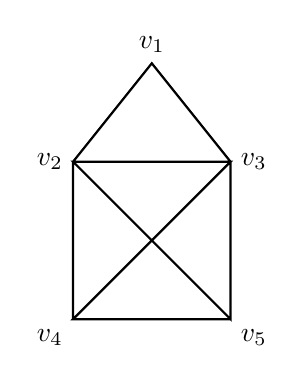
\begin{tikzpicture}[domain=0:4]
            \draw[thick,sharp corners=0pt]
            (0,0) node[anchor=north east]{$v_4$} --
            (0,2) node[anchor=east]{$v_2$} -- 
            (1,3.25) node[anchor=south]{$v_1$} --
            (2,2) node[anchor=west]{$v_3$} -- 
            (2,0) node[anchor=north west]{$v_5$} -- 
            (0,2) --
            (2,2) -- 
            (0,0) -- 
            (2,0);
        \end{tikzpicture}
    \end{minipage} %
    \begin{minipage}{.5\textwidth}
        $\begin{matrix}
            & v_1 & v_2 & v_3 & v_4 & v_5 \\
        v_1 & 0 & 1 & 1 & 0 & 0 \\
        v_2 & 1 & 0 & 1 & 1 & 1 \\
        v_3 & 1 & 1 & 0 & 1 & 1 \\
        v_4 & 0 & 1 & 1 & 0 & 1 \\
        v_5 & 0 & 1 & 1 & 1 & 0
        \end{matrix}$
    \end{minipage}%
    \newline%
    \newline%
    Codewort: $\#0100\#10111\#11011\#01101\#01110\#$
    $\rightarrow$ Buchstaben aus $\{0, 1, \#\}$
\end{example}

\begin{definition}
    Ein Alphabet $\Sigma$ ist eine endliche nicht leere Menge.
\end{definition}

\begin{example}
    \begin{align}
        \Sigma_{\text{graph}} &= \{ 0, 1, \# \} \\
        \Sigma_{\text{latein}} &= \{ a, b, c, \dots, x, y, z \} \\
        \Sigma_{\text{griech}} &= \{ \alpha, \beta, \gamma, \dots, \omega \} \\
        \Sigma_{\text{boole}} &= \{0, 1\} = \Sigma_{bin} \\
        \Sigma_{\text{dezi}} &= \{0, 1, \dots, 9\} \\
        \Sigma_{\text{unär}} &= \{1\} \\
        \Sigma_{\text{Tastatur}} &= \{a, b, c, \dots, z\} \cup \{A, B, C, \dots, Z\} \cup \{\text{ä}, \text{Ä}, \dots\} \\
        &\phantom{==} \cup \{0, \dots, 9\} \cup \{!, \backslash, \#, ;, -, ~, \dots\} \cup \{\text{␣}\}
    \end{align}
    $\hookrightarrow \emptyset, \mathbb{N}$ sind keine Alphabete
\end{example}

\begin{definition}
    Es sei $\Sigma = \{a_1, a_2, \dots, a_m\}$ ein Alphabet mit $m$ Buchstaben. Ein Wort $w$ ist eine endliche Folge von Buchstaben aus $\Sigma$, etwa:
    \[ w = a_{i1} \; a_{i2} \; \dots \; a_{in}, \quad a_{ij} \in \Sigma \]
    Die Länge dieses Wortes ist $n$ -- die Anzahl seiner Buchstaben. \\
    \\ 
    Schreibweise: $|w| = n$. \\
    Sonderfall: Das leere Wort $\lambda$ hat die Länge 0. \\
    $\Sigma^*$ bezeichnet die Menge aller (endlichen) Wörter über $\Sigma$.

    \begin{align}
        \Sigma^0 &:= \{\lambda\} \\
        \Sigma^{n+1} &:= \Sigma^n \cdot \Sigma := \{wa\;|\;w \in \Sigma^n,\;a \in \Sigma\} \\
        \Sigma^* &:= \bigcup_{n\in \mathbb{N}} \Sigma^n
    \end{align}
\end{definition}

Für die Länge gilt: $|\lambda| = 0 \quad , \quad |wa| = |w| + 1$
\[ w \in \Sigma^n \leftrightarrow |w| = n \]

\begin{remark}
    Was sind Wörter über $\Sigma_{\text{Tastatur}}$?
    \begin{itemize}
        \renewcommand{\labelitemi}{$\rightarrow$}
        \item Wörter der natürlichen Sprache
        \item Zahlen
        \item Sätze, Texte, Romane, \dots 
        \item Graphen
    \end{itemize}
    $\hookrightarrow$ Der Begriff Wort ist in der Informatik ein anderer als in der Umgangssprache. Alle Informationen, alle Daten, ... sind Wörter.
\end{remark}

\pagebreak

\subsubsection{Operationen für Wörter}
\paragraph{Konkatenation / Hintereinanderschreiben}\phantom{ }\\
Für zwei Wörter
    \begin{align*}
        u &= x_1\, x_2\, \dots\, x_n \\
        v &= y_1\, y_2\, \dots\, y_k
    \end{align*}
    mit $x_i, y_j \in \Sigma = \{ a_1, a_2, \dots, a_m \}$ ist
    \[ u \circ v := x_1\, x_2\, \dots\, x_n\  y_1\, y_2\, \dots\, y_k \]
    die Konkatenation von $u$ und $v$.\\
    Das ist damit eine zweistellige assoziative Operation: $(u\circ v)\circ w = u \circ (v\circ w)$ mit der Eigenschaft $u\circ \lambda = u = \lambda \circ u$. Das heißt $\lambda$ ist das neutrale Element.

\end{document}
